% !TEX root = ../chap2.tex

\section{Limite du modèle cinétique vers le modèle hybride}
 \label{s:limit}

Il s'agit ici d'étudier numériquement la convergence du modèle cinétique \eqref{eq:vlasov}-\eqref{eq:poisson} vers le modèle VHL \eqref{eq:vahl}, lorsque la température $T_c$ des particules froides tend vers 0. Une première étude de consistance est effectuée sur les relations de dispersion. Une seconde étude, numérique, montre la convergence de différentes quantités obtenues par les schémas proposés dans la section \ref{s:scheme}. Ces deux études complémentaires ont pour but de justifier l'utilisation de la modélisation hybride linéarisée lorsque les particules se répartissent en deux faisceaux: l'un de particules chaudes (rapides) et l'autre de particules froides (de température $T_c\ll 1$, lentes). Pour cela, le modèle cinétique \eqref{eq:vlasov}-\eqref{eq:poisson} sera initialisé avec 
\begin{equation}
  f^0(x,v) = \mathcal{M}_{1-\alpha,0,T_c}(v) + (1+\epsilon\cos(kx))\left( \mathcal{M}_{^\alpha/_2,v_0,1}(v) + \mathcal{M}_{^\alpha/_2,-v_0,1}(v) \right)
\label{eq:K:init}
\end{equation}
avec $k = 0.5$, $v_0 = 4$, $\alpha$, $x\in[0,4\pi]$, $v\in[-v_{\text{max}},v_{\text{max}}]$ avec $v_{\text{max}}=8$ et la perturbation des particules chaudes $\epsilon = 10^{-3}$.  Le paramètre $T_c$ prendra différentes valeurs selon les résultats que nous souhaitons illustrer. Comme dans la sous-section \ref{ssec:disp_appl}, on a noté  $\mathcal{M}_{\rho,u,T}(v)$ la distribution Maxwellienne :
$$
  \mathcal{M}_{\rho,u,T}(v) := \frac{1}{(2\pi T)^{\frac{1}{2}}}\exp\left(-\frac{\left|v-u\right|^2}{2T}\right)
$$

Pour la condition initiale des simulations avec le modèle hybride linéarisé \eqref{eq:vahl}, nous considérerons :
\begin{equation}
  \begin{aligned}
    u_c(x)   & = 0 \\
    f_h(x,v) & = (1+\epsilon\cos(kx))\left( \mathcal{M}_{^\alpha/_2,v_0,1}(v) + \mathcal{M}_{^\alpha/_2,-v_0,1}(v) \right)
  \end{aligned}
\label{eq:HL:init}
\end{equation}
où $k$, $v_0$, $\alpha$ et $\epsilon$ sont pris identiques au modèle cinétique, le domaine en $x$ et en $v$ reste inchangé. $E(t=0,x)$ est obtenu en résolvant l'équation de Poisson sur notre condition initiale, comme indiqué dans la proposition~\ref{p:vhl_conservation} :
$$
  \partial_x E(t=0) = (1-\alpha) + \int (1+\epsilon\cos(kx))\left( \mathcal{M}_{^\alpha/_2,v_0,1}(v) + \mathcal{M}_{^\alpha/_2,-v_0,1}(v) \right)\,\mathrm{d}v - 1
$$
\commentaire[Nicolas]{expliquer pourquoi il y a une bande jaune dans Fig. 1}
Avant une étude plus détaillée, nous donnons un premier aperçu des solutions des deux modèles pour le choix $T_c=0.05$. Sur la figure~\ref{fig:limit_vp}, sont tracées la condition initiale $f^0(x, v)$ du modèle cinétique (gauche), la solution numérique  $f(T_f=300, x, v)$ au temps final du modèle cinétique (milieu) et la solution numérique $f_h(T_f=300, x, v)$ au temps final des particules chaudes pour le modèle hybride (droite).  De plus, sur la figure \ref{fig:limit_ee_Tf300} est tracée l'évolution de l'énergie électrique $\|E(t, \cdot)\|_{L_2}$ au cours du temps pour ces deux modèles avec les mêmes paramètres numériques (échelle semi-logarithmique).
\begin{figure}[h]
  \centering
  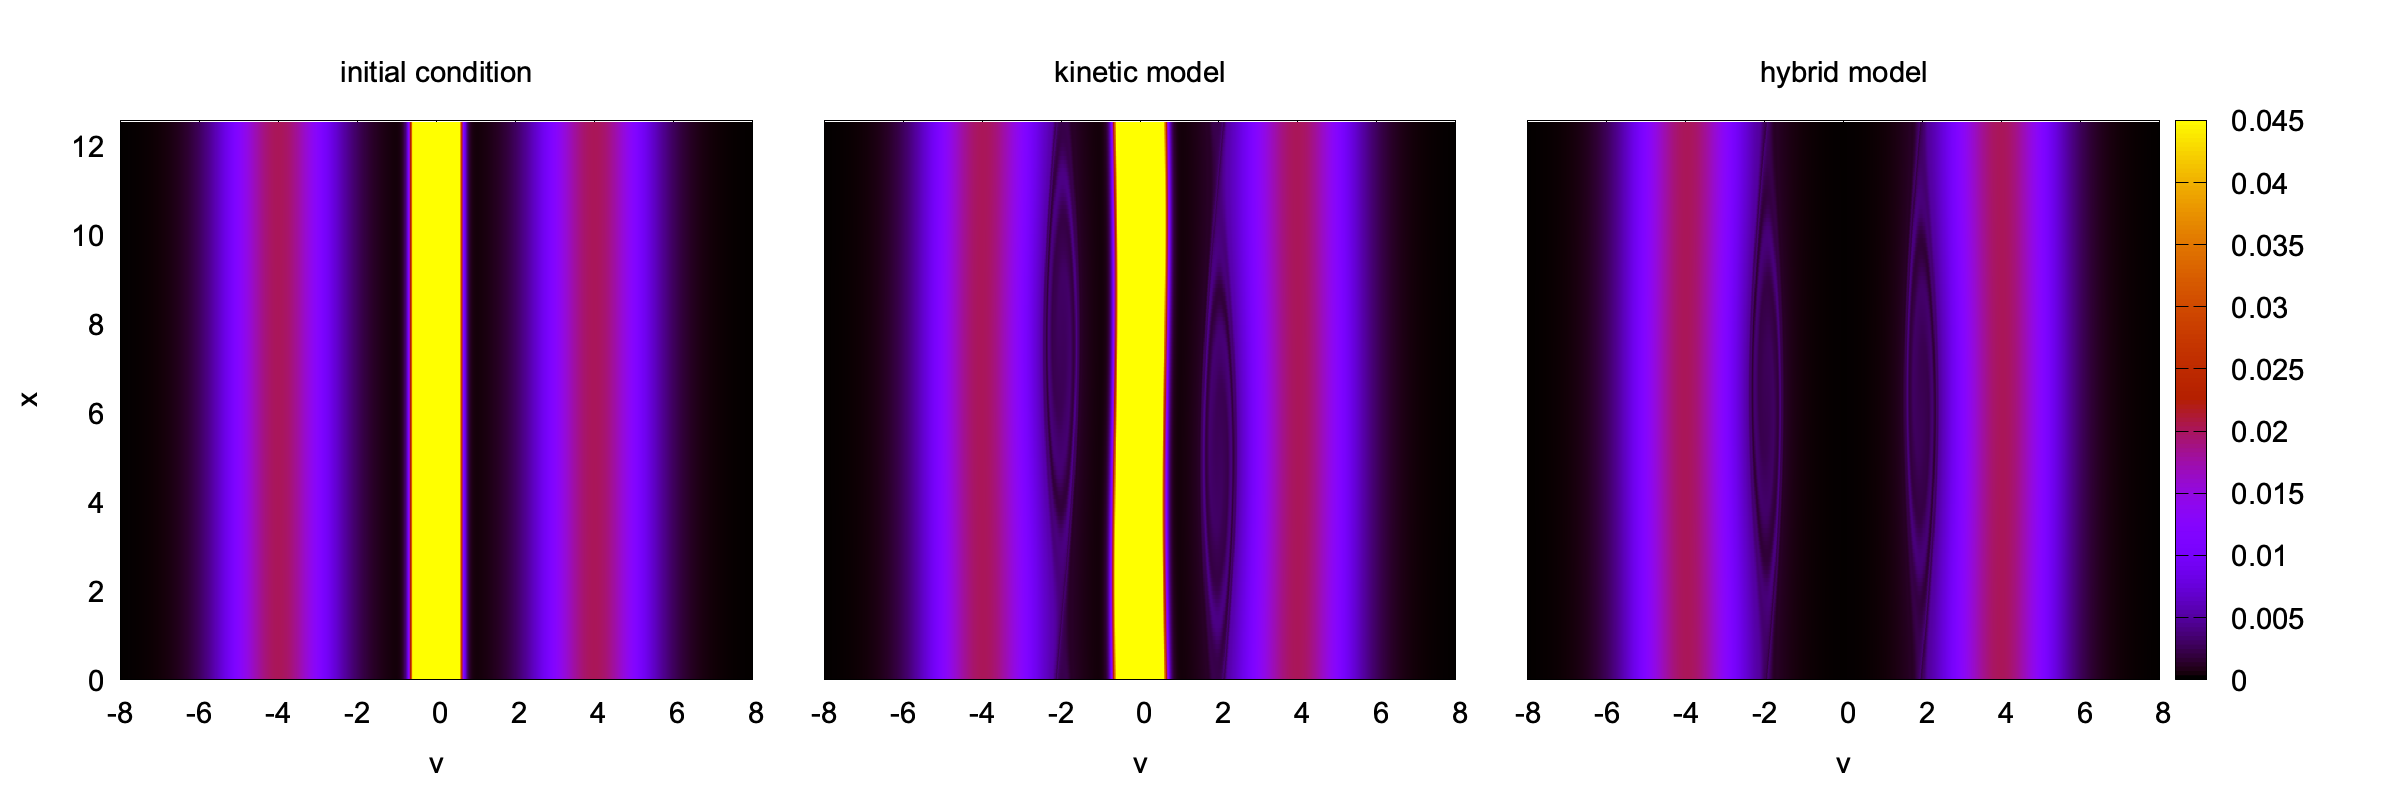
\includegraphics[width=0.9\textwidth]{\localPath/figures/limit_vp.png}
  \caption{Représentation de la condition initiale du modèle cinétique à gauche et la solution obtenue au temps final $T_f=300$ avec le modèle cinétique avec $T_c = 0.05$ (au milieu) et la densité de particules chaudes obtenue avec modèle hybride linéarisé (à droite).}
  \label{fig:limit_vp}
\end{figure}
\begin{figure}[h]
  \centering
  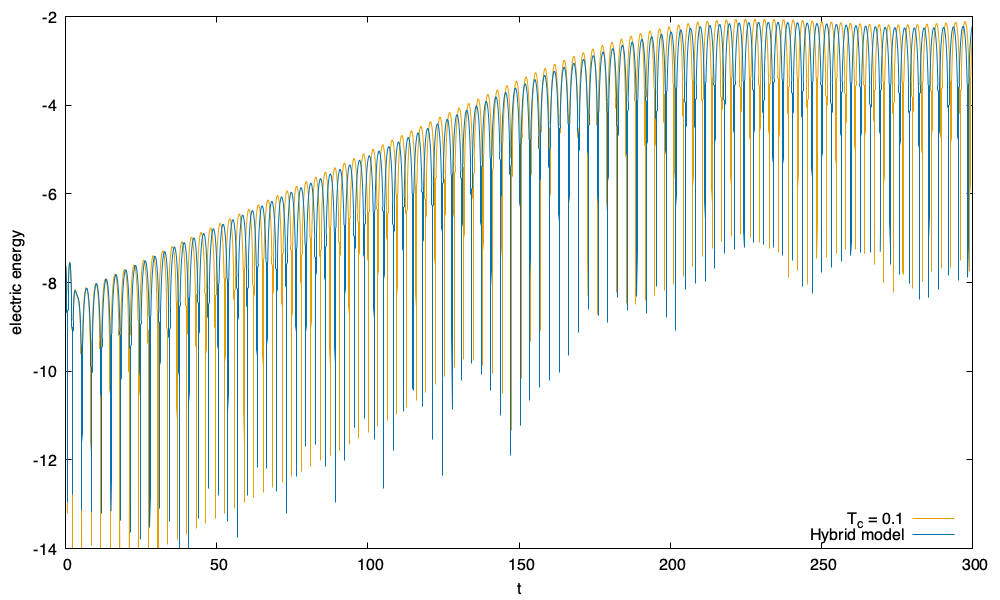
\includegraphics[width=0.8\textwidth]{\localPath/figures/limit_ee_Tf300.png}
  \caption{Énergie électrique donnée pour le modèle cinétique avec $T_c=0.05$ et le modèle hybride linéarisé.}
  \label{fig:limit_ee_Tf300}
\end{figure}
La première observation est que les résultats proches de ceux obtenus par le modèle hybride linéarisé \eqref{eq:vahl} sont très proches de ceux obtenus par le modèle cinétique \eqref{eq:vlasov}-\eqref{eq:poisson}, ce qui valide la modélisation. La perturbation des particules chaudes induit une instabilité (l'équilibre étant du type double Gaussienne) qu'on voit se développer jusqu'au temps $t=200$ (voir figure \ref{fig:limit_ee_Tf300}) et deux vortex sont alors crés autour de la vitesse $v\approx 2$, au centre desquels de fines structures se développent. 

Dans la suite, nous allons approfondir cette étude en comparant les résultats obtenus aux relations de dispersion des deux modèles puis en essayant de déterminer le domaine de validité du modèle VHL.  

%\commentaire[Anais]{(revoir un peu la rédaction de cette intro car elle ne tenait pas du tout compte de la sous-section relations de dispersion et je n'ai pas l'impression de l'avoir suffisamment modifiée)}


%----------
\subsection{Convergence en énergie totale}
%----------

Nous nous intéresserons ici à une grandeur conservée qu'est l'énergie totale, celle-ci est la somme de l'énergie cinétique et de l'énergie électrique. Pour le modèle cinétique elle se calcule comme :
$$
  \mathcal{E}_K(t) = \iint_{\Omega\times\mathbb{R}} v^2 f\,\mathrm{d}x\mathrm{d}v + \int_{\Omega} E^2\,\mathrm{d}x. 
$$
Pour le modèle VHL, l'énergie cinétique comporte deux termes, un terme fluide pour les particules froides, et un terme cinétique pour les particules chaudes :
$$
  \mathcal{E}_{VHL}(t) = \int_\Omega \rho_c u_c^2\,\mathrm{d}x + \iint_{\Omega\times\mathbb{R}}v^2f_h\,\mathrm{d}x\mathrm{d}v + \int_\Omega E^2\,\mathrm{d}x
$$

\begin{pro}
  La différence en énergie totale entre le modèle cinétique et le modèle hybride linéarisé pour des conditions initiales données par~\eqref{eq:K:init} et~\eqref{eq:HL:init} converge en $(1-\alpha)T_c|\Omega|$.
\label{p:limit:convergence}
\end{pro}
\begin{proof}
  Pour le choix de $f^0$, l'énergie totale du modèle cinétique vaut :
  $$
    \begin{aligned}
      \mathcal{E}_K(t) = \mathcal{E}_K(0) &= \iint_{\Omega\times\mathbb{R}}v^2f^0(x,v)\,\mathrm{d}x\mathrm{d}v + \int_{\Omega}E^2(t=0,x)\,\mathrm{d}x \\
                                          &= \left[ (1-\alpha)T_c + \alpha v_0^2 + \alpha \right]|\Omega|
    \end{aligned}
  $$
    On remarque que lorsque $T_c\to 0$, on obtient $\lim_{T_c\to 0}\mathcal{E}_K(t) = (\alpha v_0^2 + \alpha)|\Omega|$. L'énergie totale dans le cadre du modèle hybride se calcule comme suit :
    $$
      \mathcal{E}_{HL}(t) = \int_\Omega \rho_c^{(0)}u_c^2\,\mathrm{d}x + \iint_{\Omega\times\mathbb{R}} v^2f_h\,\mathrm{d}x\mathrm{d}v + \int_\Omega E^2\,\mathrm{d}x
    $$
    ce qui nous donne, avec le choix de condition initiale $\rho_c^{(0)} = 1-\alpha$, $u_c^0 = 0$ et $f_h^0(v) = \mathcal{M}_{^\alpha/_2,v_0,1}(v) + \mathcal{M}_{^\alpha/_2,-v_0,1}(v)$, conformément à~\eqref{eq:HL:init} :
    $$
      \mathcal{E}_{HL}(t) = (\alpha v_0^2 + \alpha)|\Omega|
    $$
    qui est bien compatible avec $\lim_{T_c\to 0}\mathcal{E}_K(t)$. De plus on peut calculer :
    $$
      \mathcal{E}_K(t) - \mathcal{E}_{HL}(t) = (1-\alpha)T_c|\Omega|
    $$
    c'est-à-dire que la convergence du modèle hybride est liée à la pression $\rho_c^{(0)}T_c$ des particules froides.
\end{proof}

Pour vérifier numériquement cette proposition nous effectuons un jeu de simulations. Le modèle cinétique de Vlasov-Poisson \eqref{eq:vlasov}-\eqref{eq:poisson} est simulé à l'aide d'une méthode en temps de type Lawson basée sur une méthode de Runge-Kutta d'ordre 4, la méthode WENO d'ordre 5 pour approcher la dérivée dans la direction $v$ et l'algorithme de FFT pour la dérivée dans la direction $x$. Il s'agit ainsi du même schéma que celui utilisé pour la fonction de distribution $f_h$ des particules chaudes du modèle hybride linéarisé. Nous choisissons la condition initiale \eqref{eq:K:init} avec $\alpha = 0.2$, $T_c \in \left\{ 0.06,0.1,0.125,0.15,0.175,0.2\right\}$, la discrétisation du domaine $\Omega = [0,4\pi]$ s'effectue avec $N_x = 135$ points, la discrétisation du domaine en vitesse $[-v_{\text{max}},v_{\text{max}}]$ nécessite de capturer la gaussienne représentant les particules froides pour différentes valeurs de $T_c$, nous choisissons donc d'adapter le nombre de points de discrétisation en vitesse $N_v$ à $T_c$, $N_v \in \left\{ 1131,1011,905,826,764,715 \right\}$, ceux-ci correspondant à environ 20 points de discrétisation pour capturer la gaussienne de température $T_c$, $N_v \approx \lceil \frac{16}{{\sqrt{T_c}}/{20}} \rceil$. Nous avons une condition CFL sur le schéma WENO utilisé dans la direction $v$, nous nous assurons d'être sous cette condition quelle que soit l'évolution de $E$ en prenant $\Delta t = 0.5\Delta v$. Ce jeu de simulations s'arrête au temps 7, or le choix des différents $\Delta t$ implique des données à des temps différents, nous choisissons d'effectuer une interpolation polynomiale de Lagrange d'ordre 5 pour exploiter les données au temps $T^\star = 6.5$. Nous obtenons ainsi l'énergie totale pour différentes températures sur la figure~\ref{fig:limit:totalenergy}, bien que le schéma de type Runge-Kutta ne conserve pas exactement l'énergie, celle-ci est bien préservée en temps court \commentaire[Nicolas]{(dire a quelle precision environ $10^{-12}$, $10^{-8}$ ?)}. Après l'interpolation au temps $T^\star = 6.5$ on obtient la convergence vers le modèle hybride sur la figure~\ref{fig:limit:totalenergy:slope} où l'on observe bien l'ordre 1 en température.
\begin{figure}[h]
  \centering
  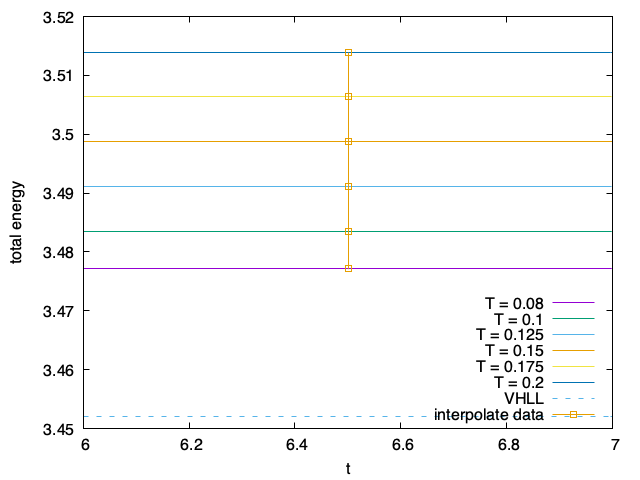
\includegraphics[width=0.8\textwidth]{\localPath/figures/limit_totalenergy.png}
  \caption{Énergie totale avec les différents modèles.}
  \label{fig:limit:totalenergy}
\end{figure}
\begin{figure}[h]
  \centering
  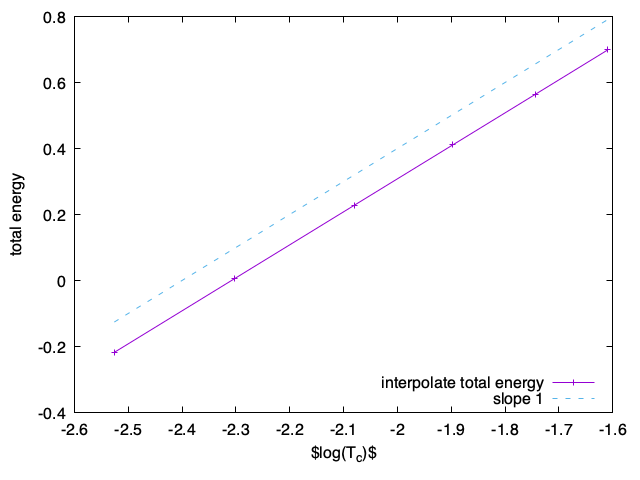
\includegraphics[width=0.8\textwidth]{\localPath/figures/limit_slope_totalenergy.png}
  \caption{Convergence de l'énergie totale du modèle cinétique vers le modèle hybride quand $T_c$ tend vers $0$.}
  \label{fig:limit:totalenergy:slope}
\end{figure}

Nous effectuons le même type d'analyse sur l'énergie électrique, à partir des données des simulations précédentes, en sachant qu'il n'existe pas de résultat théorique sur sa convergence. L'énergie électrique pour les différents choix de $T_c$ est représentée sur la figure~\ref{fig:limit:ee}\subref{fig:limit:ee:ee}, cette figure illustre mieux la nécessité d'effectuer une interpolation pour extraire les données. Une convergence est observée mais avec un ordre plus faible, environ $0.59$, que l'énergie totale sur la figure~\ref{fig:limit:ee}\subref{fig:limit:ee:slope}.
\begin{figure}[h]
  \centering
  \begin{subfigure}{0.45\textwidth}
    \centering
    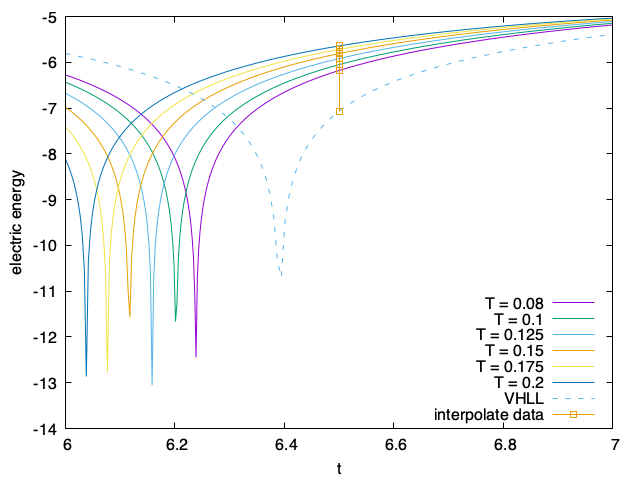
\includegraphics[width=\textwidth]{\localPath/figures/limit_ee.png}
    \caption{Énergie électrique avec les différents modèles}
    \label{fig:limit:ee:ee}
  \end{subfigure}
  \begin{subfigure}{0.45\textwidth}
    \centering
    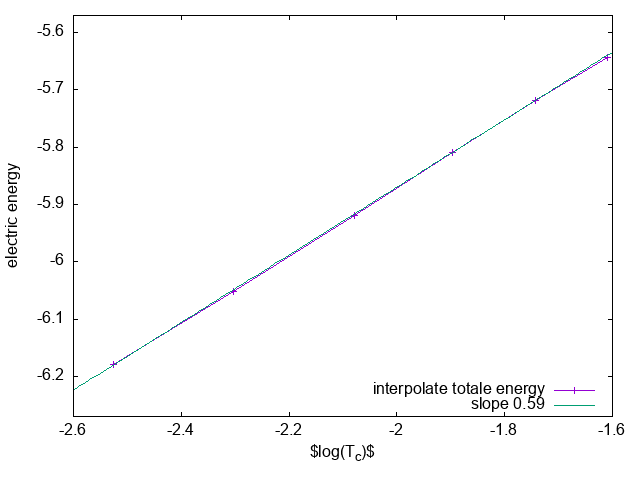
\includegraphics[width=\textwidth]{\localPath/figures/limit_slope_ee.png}
    \caption{Convergence de l'énergie électrique du modèle cinétique vers le modèle hybride quand $T_c$ tend vers $0$.}
    \label{fig:limit:ee:slope}
  \end{subfigure}
  \caption{Étude de la convergence de l'énergie électrique lorsque $T_c$ tend vers 0.}
  \label{fig:limit:ee}
\end{figure}

%----------
\subsection{Convergence en température à l'aide des relations de dispersion}
%----------

Nous étudions numériquement la convergence des racines de la relation de dispersion quant $T_c$ tend vers $0$. Pour cela, on note $D^K_{[T_c]}(\omega,k)$ la relation de dispersion du modèle cinétique \eqref{D_3bump} et $D^H(\omega,k)$ la relation de dispersion du modèle VHL \eqref{eq:D_hchyb}. Pour $k$ fixé, on note $\omega\in\mathbb{C}$ la racine de plus grande partie imaginaire. 
%Pour la relation de dispersion, nous regardons les zéros en $\omega$ de la fonction $D^K_{[T_c]}(\omega,k)$ et $D^H(\omega,k)$ à $k$ fixé par la condition initiale. Nous ne conservons que le $\omega\in\mathbb{C}$ avec la plus grande partie imaginaire. 
Cette racine est calculée numériquement à l'aide d'une méthode de Newton. On étudie maintenant la convergence des $\omega_K$ (zéro de $(D^K(\omega,k)$) vers $\omega_H$ (zéro de $(D^H(\omega,k)$). La convergence de $\omega_K(T_c)$ vers $\omega_H$ est visible sur la figure \ref{fig:omega}, où l'on représente, en échelle log-log le module de la différence des 2 zéros $\Delta \omega = |\omega_K-\omega_H|$.
\begin{figure}[h!]
  \centering
  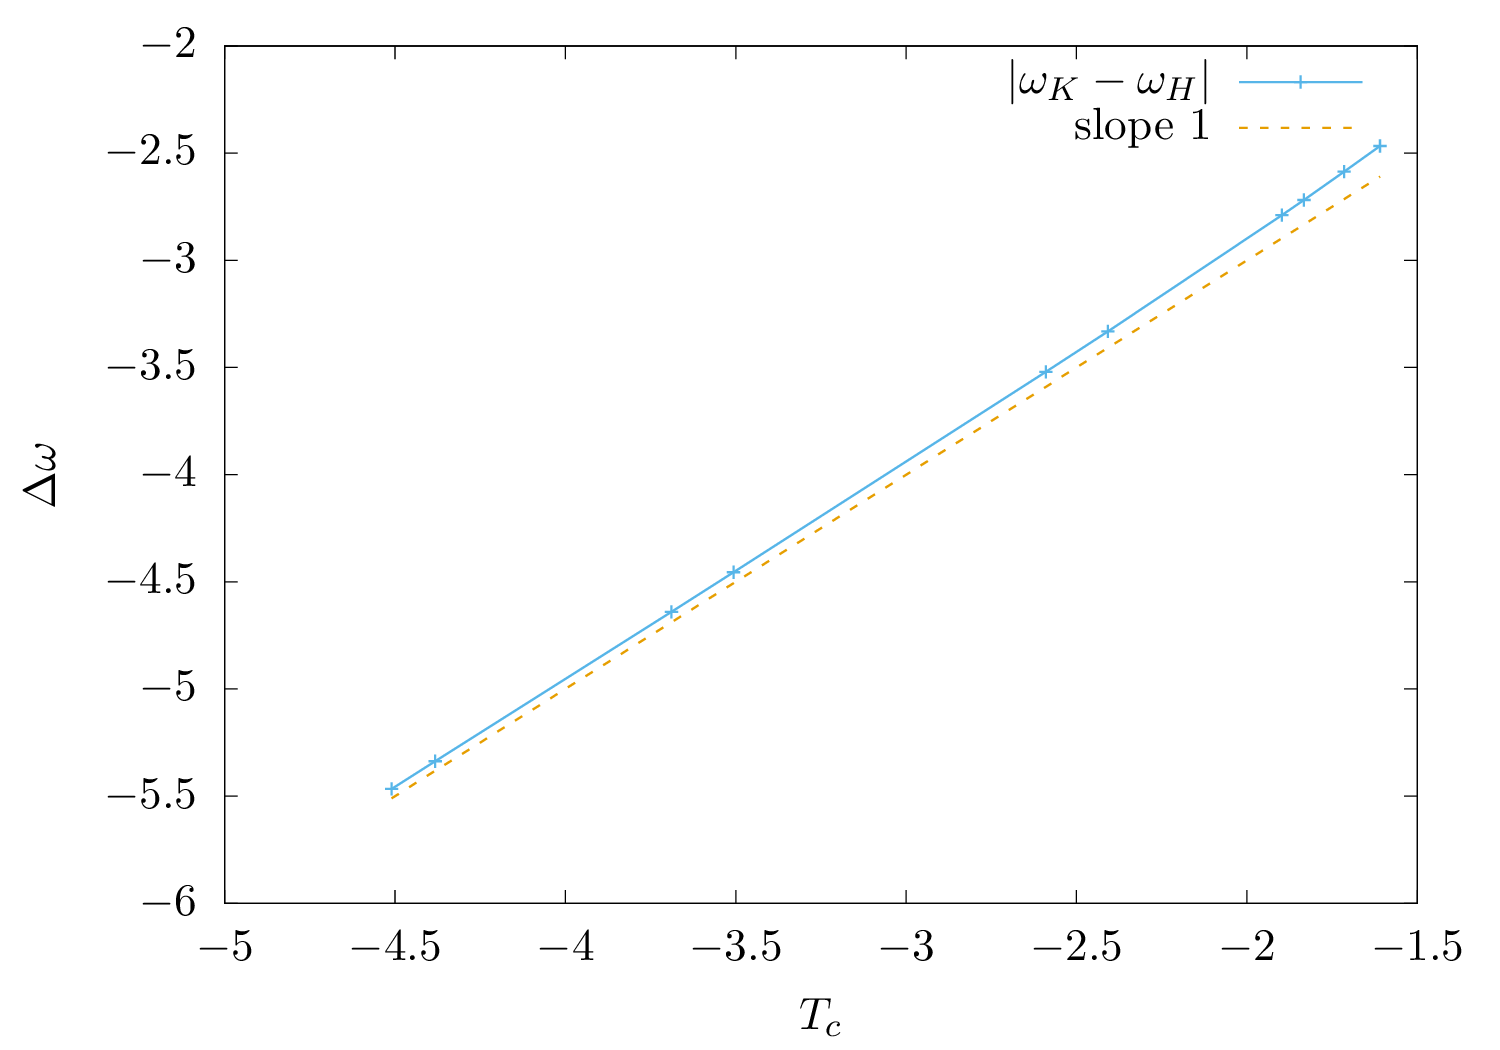
\includegraphics[width=0.8\textwidth]{\localPath/figures/omega.png}
  \caption{Convergence des zéros de la relation de dispersion cinétique vers la solution hybride}
  \label{fig:omega}
\end{figure}
On observe une convergence d'ordre $1$ en $T_c$ des zéros de la relation de dispersion, aucun argument théorique sur les fonctions holomorphes ne vient appuyer ce résultat, contrairement à ce qui a été énoncé pour l'énergie totale.

La racine de plus grande partie imaginaire permettent de valider la phase linéaire du code. Cette phase linéaire peut être rendue plus longue en considérant une valeur très faible de la perturbation $\epsilon=10^{-4}$ dans les conditions initiales~\eqref{eq:K:init} et~\eqref{eq:HL:init}. Ceci va nous permettre de vérifier non seulement le taux d'instabilité, mais aussi, grâce aux calculs de la section \ref{s:dispersion} de l'énergie électrique. Nous pouvons donc comparer pour $\alpha = 0.1$, $T_c=0.1$, $N_x=135$, $N_v=1200$, $T_f=200$ et $\Delta t = 0.5\Delta x$ ce régime linéaire sur la figure~\ref{fig:limit:ee:Tf200}\subref{fig:limit:ee:Tf200:eps10m4}. Un résultat similaire est observable pour différentes températures ainsi que sur le modèle hybride linéarisé, comme l'illustre la figure~\ref{fig:limit:ee:Tf200}\subref{fig:limit:ee:Tf200:cmp_zoom}. 
\commentaire[Nicolas]{(referer aux formules de la section \ref{s:dispersion} et donner la formule avec les valeurs de $\omega$...)}
\begin{figure}
  \centering
  \begin{subfigure}{0.8\textwidth}
    \centering
    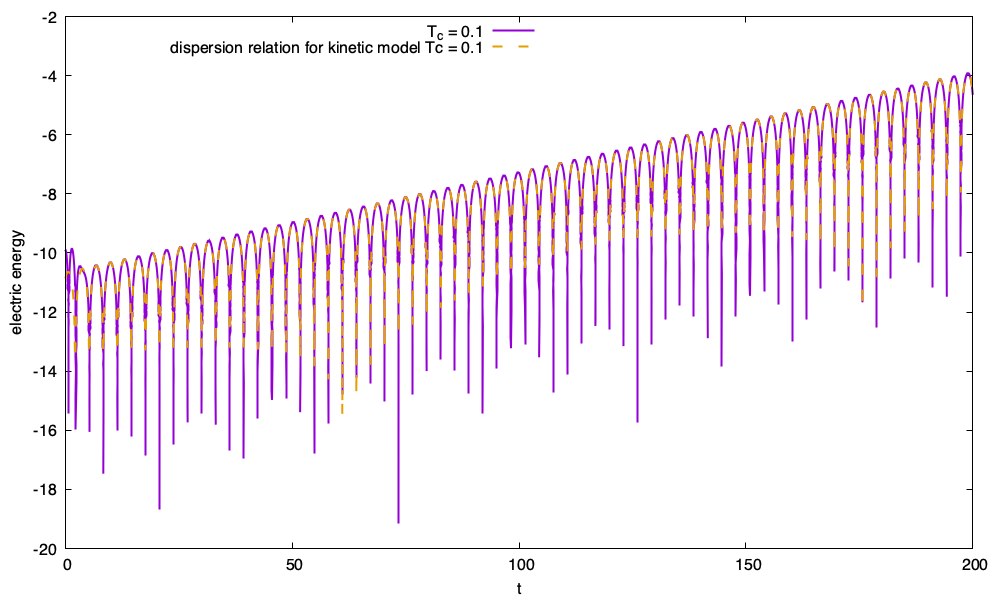
\includegraphics[width=\textwidth]{\localPath/figures/limit_ee_Tf200_eps10m4.png}
    \caption{Énergie électrique jusqu'au temps $200$ avec un régime linéaire très long, et comparaison avec les résultats données par les relations de dispersion.}
    \label{fig:limit:ee:Tf200:eps10m4}
  \end{subfigure}
  \begin{subfigure}{0.8\textwidth}
    \centering
    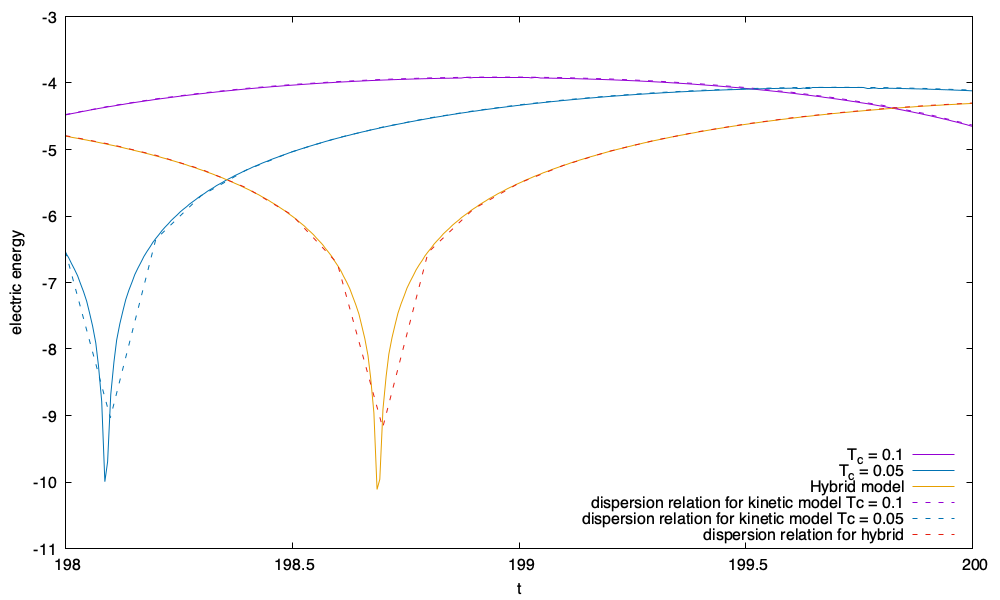
\includegraphics[width=\textwidth]{\localPath/figures/limit_ee_Tf200_cmp_zoom.png}
    \caption{Énergie électrique entre les temps $198$ et $200$ pour les températures $T_c = 0.1,0.05$ et le modèle hybride, et comparaison avec les résultats des relations de dispersion.}
    \label{fig:limit:ee:Tf200:cmp_zoom}
  \end{subfigure}
  \caption{Évolution de l'énergie électrique dans une longue phase linéaire et comparaison avec les relations de dispersion.}
  \label{fig:limit:ee:Tf200}
\end{figure}
En plus du taux d'instabilité de l'énergie électrique, il est possible à l'aide des relations de dispersion d'obtenir une très bonne approximation de l'énergie électrique dans la phase linéaire. On peut voir que l'étude des relations de dispersion ne permet pas d'obtenir des résultats fiables en début de simulation, où d'autres modes que le mode principal sont encore visibles (modes évanescents). De même, comme on peut le voir sur la figure~\ref{fig:limit_ee_Tf300}, la phase non-linéaire où l'énergie électrique atteint une saturation mélange de nombreux modes, c qui est incompatible avec l'étude du linéarisé. Néanmoins, même au temps $t\approx 200$, les résultats du code sont en excellent accord avec ceux obtenus grâce aux relations de dispersion  (voir figure \ref{fig:limit:ee:Tf200:cmp_zoom}). 


%----------
\subsection{Évolution avec la densité de particules chaudes}
%----------

Nous avons validé les modèles et les relations de dispersions lorsque la température des particules froides $T_c$ tend vers $0$, la proposition~\ref{p:limit:convergence} nous indique que la convergence s'effectue en $(1-\alpha)T_c|\Omega|$ où $\alpha$ est la densité des particules chaudes. Nous traçons sur la figure~\ref{fig:limit:slope:alpha} l'évolution du taux d'instabilité donnée par les relations de dispersions (racine de plus grande partie imaginaire) en fonction de $\alpha$ et pour différentes valeurs de $T_c$. Cette évolution est représentée pour le modèle cinétique avec différentes températures, et  pour le modèle hybride, avec comme condition initiale pour les particules chaudes :
$$
  f_h^0(x,v) = \left(\mathcal{M}_{^\alpha/_2,4,1}(v) + \mathcal{M}_{^\alpha/_2,-4,1}(v)\right)(1+\epsilon\cos\left(k x\right)), \;\; x\in [0, 4\pi]. 
$$
La condition initiale du modèle cinétique est donnée par : $f^0(x,v) = \mathcal{M}_{1-\alpha,0,T_c}(v) + f_h^0(x,v)$.
\begin{figure}[h!]
  \centering
  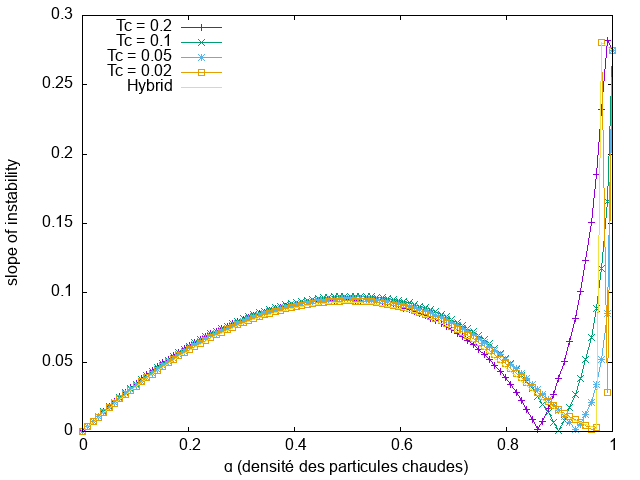
\includegraphics[width=0.8\textwidth]{\localPath/figures/limit_slope_alpha.png}
  \caption{Évolution de la pente du développement de l'instabilité (ou taux d'instabilité) donnée par les relations de dispersion en fonction de la densité de particules chaudes $\alpha$}
  \label{fig:limit:slope:alpha}
\end{figure}
On retrouve sur la figure~\ref{fig:limit:slope:alpha} la convergence en température du modèle cinétique vers le modèle hybride. Pour $\alpha=0$ la condition initiale se restreint aux particules froides, qui ne sont pas perturbées, il est donc normal d'obtenir une pente nulle ; pour $\alpha=1$, il n'y a que des particules chaudes et on retrouve l'instabilité double faisceaux (TSI) avec le bon taux d'instabilité. On peut enfin observer que pour ce choix de $T_c$, les taux d'instabilité obtenus restent proches de ceux du modèle VHL pour $0\leq \alpha \leq 0.5$ (qui correspond à une population identique de particules chaude et froide).
